In this section, user documentation and developer documentation is provided.

\section{UI Documentation}
A documentation containing screenshots with descriptions (see \autoref{fig:uiDocScreenshot}) will be at the front page of the application's github page, alongside with link to video tutorials going through previously written use cases.
The project can be found at \url{https://github.com/Palda97/LinkedPipesAndroidClient}.

\begin{figure}\centering
	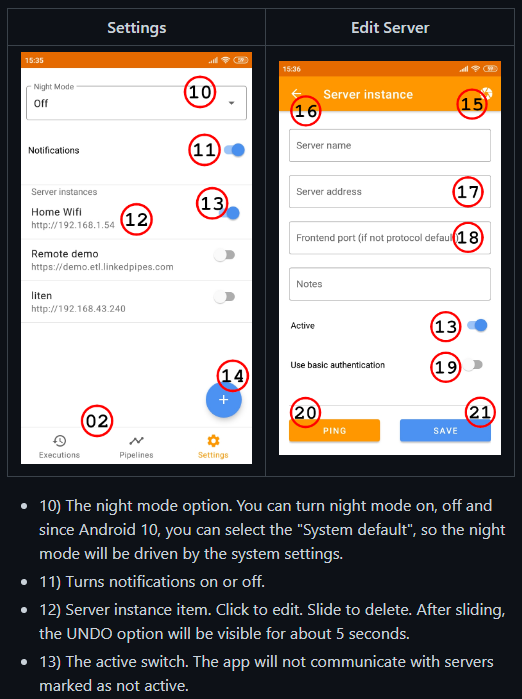
\includegraphics[width=0.87\textwidth]{pics/uiDocScreenshot.png}
	\caption[UI documentation]{UI documentation}\label{fig:uiDocScreenshot}
\end{figure}

\section{Developer documentation}
In Kotlin, there is a documenting type of comment called KDoc (see \autoref{fig:kdoc}).
With plugin called Dokka \cite{dokka}, it is possible to construct a website based on the KDoc comments, documenting the application's code.
An example of a part of a class, documented via javadoc can be seen in \autoref{fig:javadoc}.

\begin{figure}\centering
	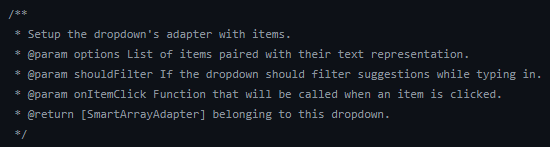
\includegraphics[width=1\textwidth]{pics/kdoccomment.png}
	\caption[KDoc comment]{KDoc comment}\label{fig:kdoc}
\end{figure}

\begin{figure}\centering
	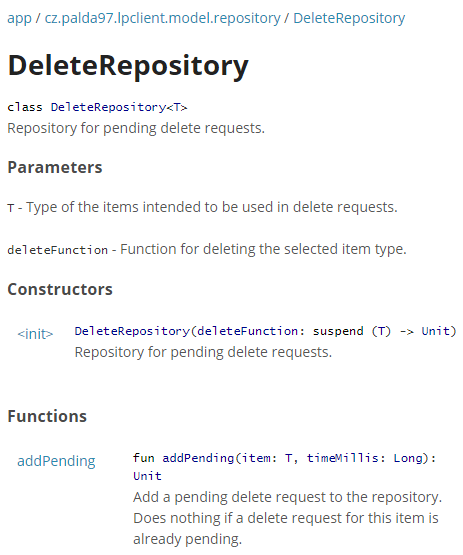
\includegraphics[width=1\textwidth]{pics/javadoc.png}
	\caption[Example of part of a javadoc page]{Example of part of a javadoc page}\label{fig:javadoc}
\end{figure}

The second part of developer documentation will be written by hand, explaining the internal operations from a greater distance, so other developers can have a more bearable understanding of the application when they follow up on development.
Part of the handwritten developer documentation can be seen in \autoref{fig:developerdocumentation}

\begin{figure}\centering
	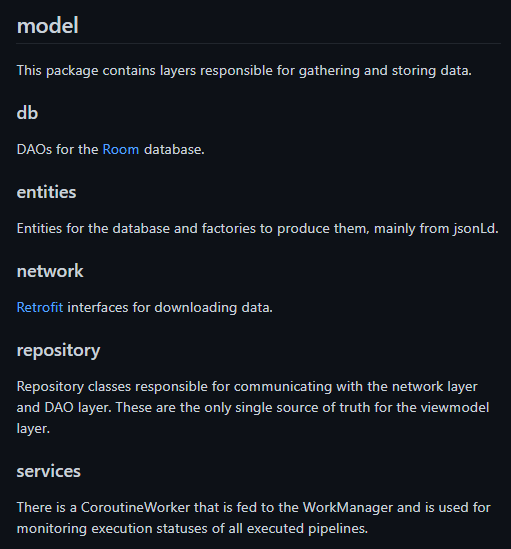
\includegraphics[width=1\textwidth]{pics/developerDocumentation.png}
	\caption[Part of the handwritten developer documentation]{Part of the handwritten developer documentation}\label{fig:developerdocumentation}
\end{figure}

Link to developer documentation will be accessible from the application's github page.
